\newpage
\subsubsection{ALS XZ}
Die Technik \textit{ALS XZ} ist die einfachste Unterart der \textit{Almost Lockes Sets}. Man sucht zwei \textit{ALS} mit einem \textit{RCC}. Dieser wird x genannt. Wenn beide \textit{ALS} noch einen gemeinsamen Kandidaten z besitzen, der kein \textit{RCC} ist, dann kann z aus allen Zellen gelöscht werden, die nicht zum \textit{ALS} gehören und die alle Instanzen von z in beiden \textit{ALS} sehen. Das funktioniert, da durch x ein \textit{ALS} zum \textit{Locked Set} wird. Da in beiden \textit{ALS} die Ziffer z vorkommt wird diese auf ein \textit{ALS} beschränkt. Das bedeutet, dass z in genau einem \textit{ALS} vorkommt und daher können alle Kandidaten gelöscht werden, die von allen Instanzen gesehen werden.

\begin{figure}[h]
\begin{center}
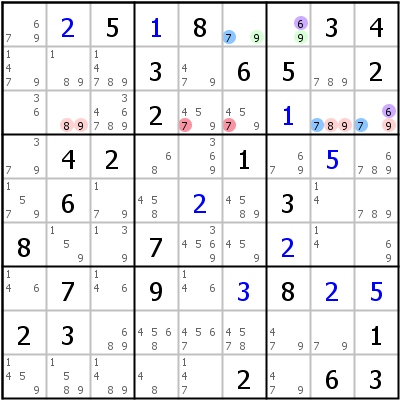
\includegraphics{./img/ALS_XZ.png}
\caption{ALS XZ}
\end{center}
\end{figure}

\noindent In \textbf{Abbildung 2.20} sehen wir die beiden \textit{ALS} einmal in Zeile 4 Spalte 2 und 4 mit den Kandidaten 4, 5 und 8 und das zweite in Zeile 6 Spalte 2, 7 und 9 mit den Kandidaten 3, 4, 5 und 6. Der \textit{RCC} ist hier die Ziffer 5, da alle Instanzen in beiden \textit{ALS} in Spalte 2 liegen. Ausserdem kommt in beiden \textit{ALS} die Ziffer 4 vor, die aber kein \textit{RCC} ist, da sich zum Beispiel z4s4 und z8s9 nicht sehen können. Nun können alle Zellen die Ziffer 7 von ihren Kandidatenlisten, die alle Instanzen der Ziffer 7 in beiden \textit{ALS} sehen, was in z8s4 der Fall ist.